\chapter{Arquitetura do Projeto}
\label{arq-cap}

\section{Sensor}
\label{sensor-cap}

\section{Preparação de dados}

\section{Apresentação de dados}

O sistema proposto para medir o tráfego de pessoas dentro de uma determinada
zona a partir de sinais Wi-Fi é baseado no esquema da \autoref{esquema-geral},
que será explicado nos itens a seguir:

\begin{figure}[!h]
  \caption{\label{esquema-geral}Arquitetura geral do sistema}
  \begin{center}
    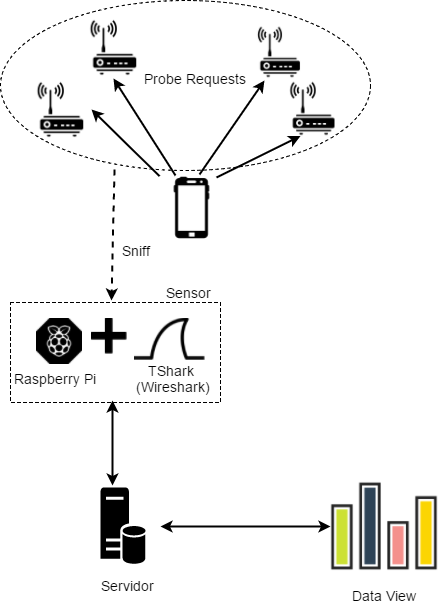
\includegraphics[width=0.50\textwidth]{img/esquema_geral.png}
  \end{center}
  \legend{Fonte: Elaborada pelas autoras.}
\end{figure}

\section{Detalhamento de processos}
O esquema da \autoref{esquema-geral} expõe de maneira mais abstrata o
funcionamento do sistema de medição de tráfego. Já o diagrama de fluxo da
\autoref{diagrama-fluxo} apresenta os processos, entidades externas e
repositórios de armazenamento que compõe o sistema.

\begin{figure}[!h]
  \caption{\label{diagrama-fluxo}Processos e entidades do sistema}
  \begin{center}
    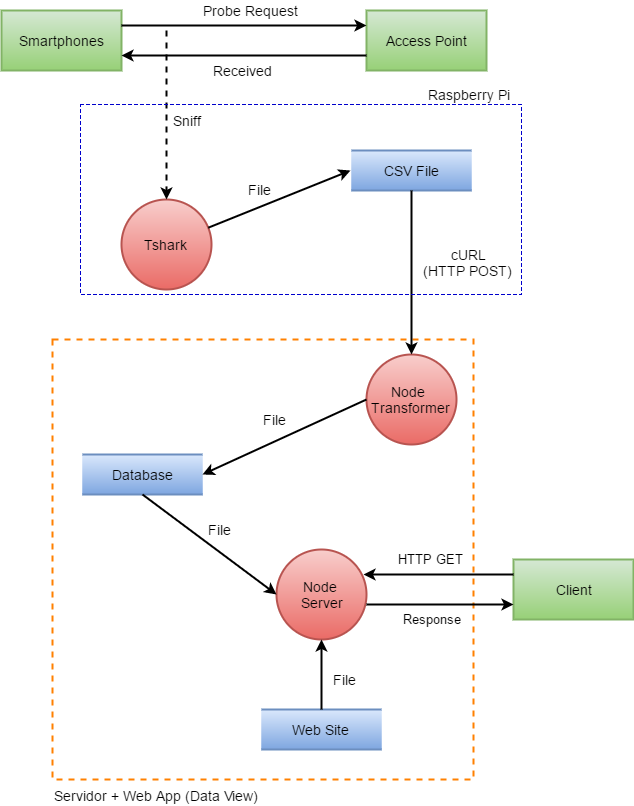
\includegraphics[width=0.70\textwidth]{img/diagrama_fluxo.png}
  \end{center}
  \legend{Fonte: Elaborada pelas autoras.}
\end{figure}

\section{Servidor}
O servidor que atenderá ao Web App será baseado em Node.js. Ele possui duas partes principais que serão apresentadas a seguir.

\subsection{Node Transformer}
\label{node-transformer}
Após converter os dados do pacotes recebidos para um arquivo, o
Raspberry Pi dá um cURL POST (HTTP POST através do terminal) de tempos em tempos
para enviar o arquivo daquela sessão ao servidor. No servidor, o módulo
node transformer particionará o arquivo (segundo alguns campos) em outros
arquivos .JSON, que serão salvos no banco de dados.

\subsection{Node Server}
 A partir dos arquivos .JSON citados no item anterior e um Web Site base (HTML,
 CSS, Javascript), o módulo Node Server responde (Response) à requisição do
 cliente (HTTP GET) e apresenta-o os dados capturados.

\section{Data View}
O Data View é a parte do Web App responsável por apresentar os dados capturados
de maneira clara e legível. Para isso, a biblioteca D3.js \cite{D32017} será
utilizada para a plotagem de gráficos a partir dos arquivos .JSON.

\section{Protótipo}
Como apresentação parcial e prova de funcionamento dos componentes anteriores, o protótipo desenvolvido é baseado no sensor.
Trata-se de um Raspberry Pi equipado com um adaptador Wi-Fi que consegue capturar, analisar e exportar os pacotes \emph{probe request} para um arquivo, que será enviado ao servidor. Essa etapa é garantida pelo protocolo de análise de rede Tshark.

Os comandos do Tshark que capturam os pacotes provenientes dos dispositivos móveis são realizados através de um servidor local feito em Node.js.

\begin{figure}[!h]
  \caption{\label{prototipo-app}Protótipo do sistema}
  \begin{center}
    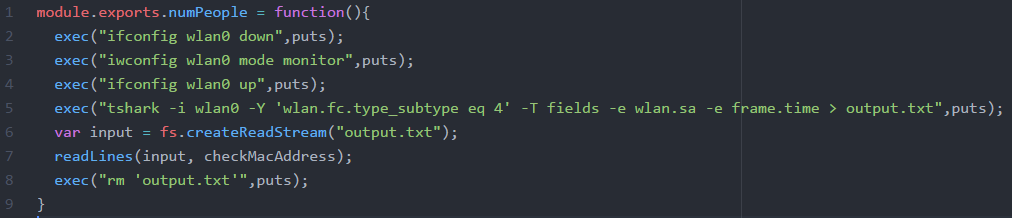
\includegraphics[width=1.0\textwidth]{img/prototipo-app.png}
  \end{center}
  \legend{Fonte: Elaborada pelas autoras.}
\end{figure}

A \autoref{prototipo-app} apresenta o código de um módulo Node.js que
assemelha-se com a função que será desempenhada pelo Node Transformer
(\autoref{node-transformer}). Esse módulo é chamado no servidor. As linhas que
possuem o comando ``exec'' executam comandos diretamente no terminal do sistema
operaciomal. Nas linhas 2-4, habilita-se o adaptador de rede para o modo
monitor. Na linha 5, o comando Tshark rodado representa:
\begin{center}
\emph{tshark -i wlan1 -a duration:40 -Y ``wlan.fc.type\_subtype eq 4'' -T fields -e wlan.sa}
\end{center}


\begin{itemize}
  \item \textbf{wlan0}: interface de rede que indica a antena Wi-Fi;
  \item \textbf{wlan.fc.type\_subtype eq 4}: indica que só pacotes \emph{probe request} devem ser capturados;
  \item \textbf{wlan.sa}: representa o \emph{source address} ou endereço MAC do dispositivo que enviou o pacote;
  \item \textbf{frame.time}: representa a hora, dia e ano em que o pacote foi capturado.
\end{itemize}

Em seguida no código, o arquivo exportado pelo Tshark é lido através de um \emph{stream}. A função ``readLines()''
na linha 7, lê o arquivo linha por linha, identificando os endereços MAC diferentes e adicionando-os a uma lista.
Então, nessa própria função é mostrado no terminal (``console.log(list)''), quantas pessoas foram contadas, ou em outros termos,
quantos dispositivos diferentes foram detectados. Na \autoref{arquivo-pacotes}, mostra-se o arquivo com os pacotes
capturados. Na \autoref{exec-bash} apresenta-se o que a execução da aplicação feita gerou, no caso, detectou
4 pessoas nas proximidades.

\begin{figure}[!h]
  \caption{\label{arquivo-pacotes}Arquivo com pacotes capturados}
  \begin{center}
    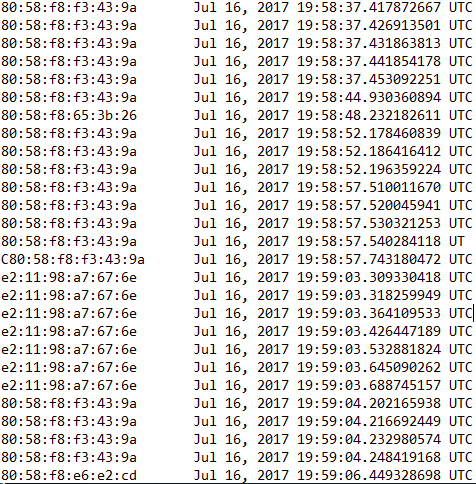
\includegraphics[width=0.70\textwidth]{img/packets.png}
  \end{center}
  \legend{Fonte: Elaborada pelas autoras.}
\end{figure}

\begin{figure}[!h]
  \caption{\label{exec-bash}Resultado da execução da aplicação}
  \begin{center}
    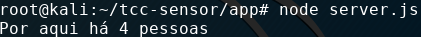
\includegraphics[width=1.0\textwidth]{img/bash.png}
  \end{center}
  \legend{Fonte: Elaborada pelas autoras.}
\end{figure}
